\section{Internet of Things -- IoT}
\begin{itemize}
	\item Definition: a system of interrelated devices with unique identifiers, which can transfer data over network without human-human/human-computer interaction.
	\item devices: mobile, alexa, sensors, vehicles, actuators, industrial machines, sweeping robots blabla.
	\item applications: smart home/parking/health/city/agriculture blabla.
	
	 
\end{itemize}

\subsection{IoT Architectures}

\begin{itemize}
	\item \textbf{cloud} architecture: devices $\xrightarrow[]{\text{IoT network}}$ Gateway $\xrightarrow[]{\text{WAN}}$ IoT platform on cloud data center
	
	
	\item \textbf{edge} architecture: devices $\rightarrow$ \textbf{edge computers} $\xrightarrow[]{\text{WAN}}$ IoT platform on cloud data center
	\begin{itemize}
		
		\item \textbf{Preprocessing} computation nearer to devices (cloud too far \& slow). eg: aggregation, filtering on threshold, analysis. 
		
		$\rightarrow$ smaller latency, saves bandwidth
		\item use-case: compute devices on car/service robots(real-time)
	\end{itemize}
	
	\item \textbf{fog} architecture: devices $\xrightarrow[]{\text{IoT network}}$ Gateway $\rightarrow$ \textbf{islands of coupled edge devices} $\xrightarrow[]{\text{WAN}}$ IoT platform on cloud data center
	\begin{itemize}
		\item extension of edge architecture: an extra layer with coupled edge systems.
		\item \textbf{distributed loaction awared shared} infrastructure
		\item characteristics: contextual location awareness, low latency, heterogeneity(edge/accelerator/server for different processing purposes), real-time interactions, interoperatbility of different providers, scalability
	\end{itemize}
\end{itemize}

\subsection{IoT Network}
\begin{itemize}
	\item wireless, connects devices to a gateway
	\item \textbf{Low Power Wide Area Network(LPWAN)}: long distance, low power consuming for battery-charged devices
	
	
	\item \textbf{Long Range Wide Area Network(LoRaWAN)}: 
	\begin{itemize}
		\item low frequency wave --> \textbf{long distance} >10km, for transferring \textbf{small messages}
		\item \textbf{range overlapping}: device can communicate with server A \& B $\rightarrow$ \textbf{message duplication} at infrastructure $\rightarrow$ \textbf{De-duplication} necessary
		\item based on \textbf{Chirp Spread Spectrum} modulation: spreading factor $\uparrow$, transmitting speed of a symbol $\downarrow$, amount of data transmitted$\downarrow$, payload size $\downarrow$
		\item Use-case: The Things Network -- a global open LoRaWAN network
	\end{itemize}
	
\end{itemize}

\subsubsection{The Things Network}
\begin{itemize}
	\item one network for the whole world.
	\item long range gateways, for low power devices.
	\item intermediate between low power devices and IoT infrastructures, servers, apps, etc.
	\item Architecture \& Data Flow: a distributed system
	\begin{itemize}
		\item Gateway: distributed over the world, \textbf{devices} connect to \textbf{gateway}. 
		\item Router: each \textbf{gateway} is connected to a \textbf{router}. Messages are forward to router or back.
		\item Broker: \textbf{router} communicates to \textbf{broker}. Broker brings application and devices together, it forwards the message to the corresponding application.
		\item network server: maintains the state of network, mapping between short address of device and network session key, identification of device
		\item discovery: component discovery of routers and handlers.
	\end{itemize}
	\begin{figure}[H]
		\centering
		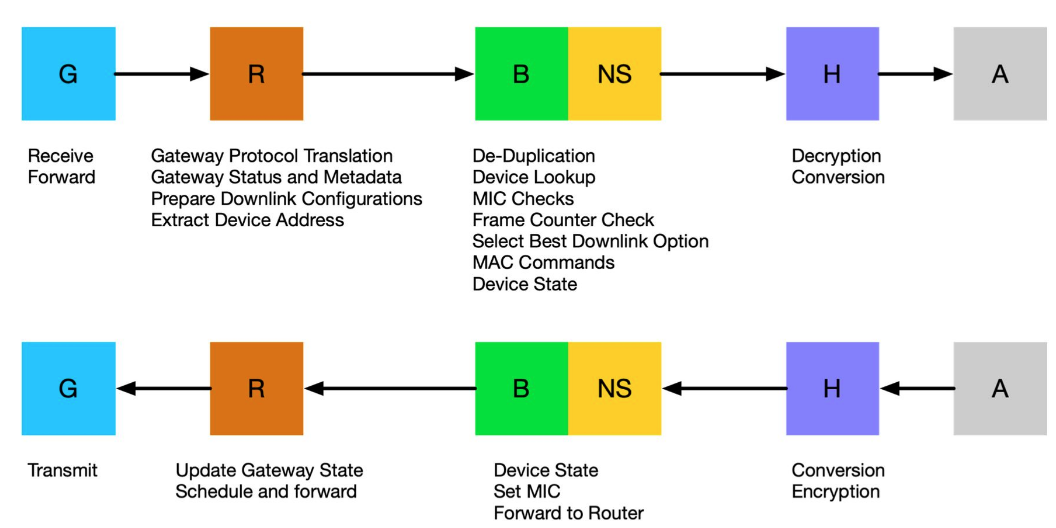
\includegraphics[width=0.8\textwidth]{ttn.png}
	\end{figure}
\end{itemize}